\documentclass{standalone}
\usepackage{xcolor}
\usepackage{verbatim}
\usepackage[T1]{fontenc}
\usepackage{graphics}
\usepackage{hyperref}
\newcommand{\code}[1]{\texttt{#1}}
\newcommand{\R}{R}
\newcommand{\pkg}[1]{#1}
\newcommand{\CRANpkg}[1]{\pkg{#1}}%
\newcommand{\BIOpkg}[1]{\pkg{#1}}
\usepackage{amsmath,amssymb,array}
\usepackage{booktabs}
\usepackage{subcaption}
\usepackage{tikz}  
\usetikzlibrary{shapes.geometric, arrows.meta, positioning}

\begin{document}
\nopagecolor
\centering

\label{fig:robust-mahalanobis-workflow}
\vspace{0.5em}
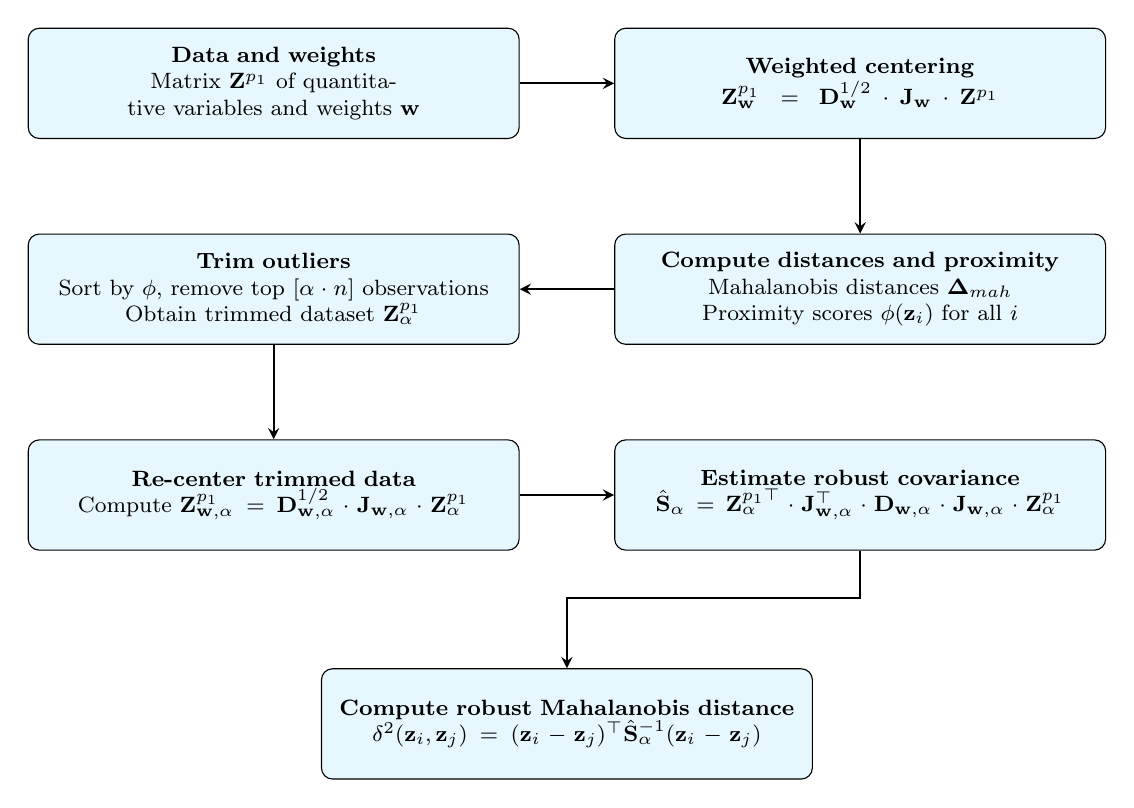
\begin{tikzpicture}[node distance=1.2cm and 1.2cm, >=stealth]
\tikzset{
  box/.style={rectangle, draw, text width=6cm, align=center, rounded corners,
              minimum height=1.4cm, fill=cyan!10, font=\footnotesize},
  arrow/.style={->, thick}
}
\node[box] (A) {
 \textbf{Data and weights} \\
 Matrix $\mathbf{Z}^{p_1}$ of quantitative variables and weights $\mathbf{w}$
};
\node[box, right=of A] (B) {
  \textbf{Weighted centering} \\
  $\mathbf{Z}_{\mathbf{w}}^{p_1} = \mathbf{D}_{\mathbf{w}}^{1/2} \cdot \mathbf{J}_{\mathbf{w}} \cdot \mathbf{Z}^{p_1}$
};
\node[box, below=of B] (C) {
  \textbf{Compute distances and proximity} \\
  Mahalanobis distances $\mathbf{\Delta}_{mah}$ \\
  Proximity scores $\phi(\mathbf{z}_i)$ for all $i$
};
\node[box, left=of C] (D) {
  \textbf{Trim outliers} \\
  Sort by $\phi$, remove top $[\alpha \cdot n]$ observations \\
  Obtain trimmed dataset $\mathbf{Z}_{\alpha}^{p_1}$
};
\node[box, below=of D] (E) {
  \textbf{Re-center trimmed data} \\
  Compute $\mathbf{Z}_{\mathbf{w},\alpha}^{p_1} = \mathbf{D}_{\mathbf{w},\alpha}^{1/2} \cdot \mathbf{J}_{\mathbf{w},\alpha} \cdot \mathbf{Z}_{\alpha}^{p_1}$
};
\node[box, right=of E] (F) {
  \textbf{Estimate robust covariance} \\
 $\hat{\mathbf{S}}_\alpha = \mathbf{Z}_{\alpha}^{p_1\top} \cdot \mathbf{J}_{\mathbf{w},\alpha}^{\top} \cdot \mathbf{D}_{\mathbf{w},\alpha} \cdot \mathbf{J}_{\mathbf{w},\alpha} \cdot \mathbf{Z}_{\alpha}^{p_1}$
};
\path (F) -- (E) coordinate[midway] (midpoint);
\node[box, below=2.2cm of midpoint] (G) {
  \textbf{Compute robust Mahalanobis distance} \\
  $\delta^2(\mathbf{z}_i,\mathbf{z}_j) = (\mathbf{z}_i-\mathbf{z}_j)^\top \hat{\mathbf{S}}_\alpha^{-1} (\mathbf{z}_i-\mathbf{z}_j)$
};
\draw[arrow] (A) -- (B);
\draw[arrow] (B) -- (C);
\draw[arrow] (C) -- (D);
\draw[arrow] (D) -- (E);
\draw[arrow] (E) -- (F);
\draw[arrow] (F.south) -- ++(0,-0.6) -| (G.north);
\end{tikzpicture}
\end{document}
